\chapter{Introdução}
\label{cap:introducao}

Cada vez mais à tecnologia avança numa velocidade impressionante. Com esse avanço se tornou possível ter computadores com um grande poder de processamento à um menor custo e ocupando menos espaço. Com isso, algoritmos complexos de inteligência artificial realizam seus cálculos muito mais rápido, além de que, com o tempo, eles foram se tornando cada vez mais robustos \cite{rodrigues2017fundamentos}. 

A \acrlong{IA} (IA) vem evoluindo muito desde à criação do seu conceito, em 1956. Inicialmente, IA era utilizada apenas para à resolução de problemas simples e repetitivos, com aplicação de regras lógicas. Porém, com a chegada da Aprendizagem Profunda (\textit{Deep Learning}) os algoritmos passaram a poder realizar tarefas mais complexas como reconhecimento de fala e classificação de imagens. \cite{goodfellow2016deep}

Outro ramo que vem apresentando um notório crescimento é a industria automobilística. No brasil, ela representa 18,2\% da economia nacional \cite{estadao}, segundo dados de 2011. À adoção de padrões de qualidade, o aumento do nível de exigência dos consumidores e à concorrência do mercado são fatores que impactam diretamente na necessidade de inovação dos veículos produzidos, estimulando o investimento em novas tendências tecnológicas. Entre todas essas tendências, é possível afirmar que à condução autônoma é a mais revolucionária da atualidade. Ela mudará toda à concepção de locomoção veicular que temos. \cite{rodrigues2017fundamentos}

O imenso poder computacional, os complexos algoritmos de inteligência artificial da atualidade e aprendizagem profunda abriu espaço para um sonho antigo ser desenvolvido: os carros autônomos. 
%Com o uso da linguagem \textit{python}, algoritmos de \textit{Deep Learning} e ROS, são adaptados nesse projeto um algoritmo para automatizar a movimentação da Plataforma Robótica Jaguar em duas pistas da Unifor.
Com o uso da linguagem \textit{python}, algoritmos de \textit{Deep Learning} e ROS, é adaptado para a plataforma Robótica Jaguar o algoritmo utilizado no projeto do \textit{Nanodegree} de carros autônomos da Udacity.

\section{Motivação}
\label{sec:motivacao}

Segundo Elon Musk, CEO da \textit{Tesla Motors}, em 2020 já teremos carros autônomos em circulação \cite{elonmusk}, porém o Brasil se encontra em 17º no rank divulgado pelo G1 \cite{brasilutimorank} de países mais aptos à receber à tecnologia, apesar de ter uma excelente aceitação pelos brasileiros, até maior que japoneses. 

As pesquisas divulgadas pelo G1 \cite{brasilutimorank} mostram o quão grande é à dificuldade de aplicação de tecnologia no Brasil. Segundo o rank divulgado pela KPMG \cite{brasilutimorank}, o país ocupa à última posição no rank de política e legislação e o penúltimo no rank de infraestrutura. Isso mostra que, apesar do país ter bastante dificuldades governamentais para a aplicação e desenvolvimento do projeto, não faltam pessoas querendo adquirir essa tecnologia e à corrida para o desenvolvimento desses veículos no país já começou. 

Projetos como o Smart Camaro, IARA, caRINA, e Wally, mostrados na Figura \ref{carrosautonomos} \cite{carroautonomobrasil} já estão em desenvolvimento nas universidades do pais, porém é necessário conhecimentos profundos em ROS (\acrlong{ROS}), programação em C++ e Python, fusão de sensores, visão computacional, programação em GPU (\acrlong{GPU}), além de entendimento sobre \textit{hardware}.

	\begin{figure}[H]
		\centering
		\Caption{\label{carrosautonomos} Smart Camaro, IARA, caRINA, e Wally em ordem}
		\UNIFORfig{}{
			\fbox{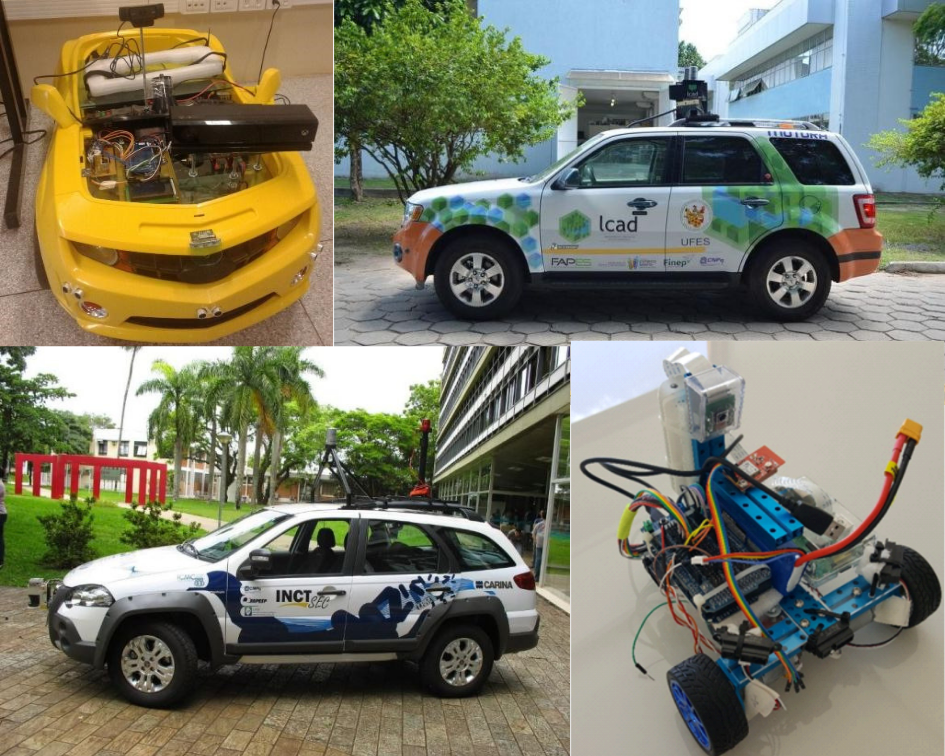
\includegraphics[width=15cm]{fig/carrosAutonomo.png}}
		}{
			\Fonte{\cite{carroautonomobrasil}}
		}	
\end{figure}

Então o maior motivador para o desenvolvimento desse trabalho é iniciar pesquisas de desenvolvimento na área de carros autônomos, pois no Brasil é uma área ainda pouco explorada, porém com um imenso potencial no qual diversas empresas Além da \textit{Tesla Motors} \cite{empresasenvolvidascomcarrosautonomos} já iniciaram pesquisa e desenvolvimento na área.

\section{Objetivos}
\label{sec:objetivos}

\subsection{Objetivo Geral}
\label{sec:objetivo-geral}

Adaptar o algoritmo do projeto \textit{Car Behavioral Cloning} para Plataforma Robótica Jaguar utilizando apenas uma câmera e utilizar imagens capturadas por ela para treinar o algoritmo de \acrlong{IA} e fazer com que o Jaguar pilote de forma autônoma.


\subsection{Objetivos Específicos}
\label{sec:objetivos-especificos}

\begin{enumerate}
\item Instalar o ROS \textit{Kinetic} no Ubuntu de Versão 16.04 LTS, criar o \textit{Workspace} e instalar todos os pacotes;
\item Instalação do Python 3.5.2 e bibliotecas para ambas as versões do Python 2.7 e 3.5.2;
\item Alterar as configurações de rede do computador para conectar à máquina com o Jaguar;
\item Obter as imagens e comandos de direção e velocidade do treino nas pistas;
\item Pilotar o Jaguar em pelo menos duas pistas em diferentes direções;
\item Treinar o algoritmo para o controle autônomo da Plataforma Robótica Jaguar com diferentes parâmetros;
\item Testar os modelos criados nas pistas utilizadas para o treinamento;
\item Avaliar o desempenho do Jaguar nas diferentes pistas, em diferentes direções e com diferentes padrões de treinamento e tirar uma conclusão dos resultados;
\end{enumerate}





\begin{enumerate}
\item Instalar o ROS em no sistema operacional Ubuntu;
\item Adaptar o algoritmo do projeto \textit{Car Behavioral Cloning} para utilizar somente uma câmera;
\item Desenvolver um programa em python que receba as imagens da câmera Jaguar, os dados de aceleração e angulação do robô e salve tudo em arquivo \textit{.csv}:
\item Criar um modelo de Rede Neural com o 
\end{enumerate}